\section{Introduction}
The semiconductor industry keeps seeking for reducing the design time and efforts in modern integrated circuit implementation, which often incorporates billions of transistors. 
Among the entire design flow, back-end design involving the physical implementation takes a significant portion of the design time.
Routing is known as the most complex and time-consuming stage in the back-end design flow due to its high complexity and enormous solution space for the very large-scale integration (VLSI) routing problem,
To the escalating challenges posed by exponential growth in System-on-Chip (SoC) design complexity under post-Moore's Law paradigms, the open-source EDA flow ''OpenROAD'' has emerged as a cutting-edge solution for complete RTL-to-GDSII implementation. 


And compared with global routing, detailed routing is the main time bottleneck in this stage, due to strict DRC adherence, larger search space, dynamic data management, manufacturing variability handling, and toolchain interoperability issues. These factors increase computational complexity and time.
TritonRoute, as the CPU-driven routing engine within the state-of-the-art open-source RTL-to-GDSII flow, delivers design-rule-clean routing solutions for advanced technology nodes at 16nm and below. 
While this methodology demonstrates robust capability in resolving complex multi-constrained routing problems with high solution quality, its inherent computational inefficiency presents a significant bottleneck that markedly impacts turnaround time.

To accelerate routing, existing approaches primarily focus on utilizing partition-based multithreaded CPUs or GPU-accelerated architectures. 
However, these methods exhibit diminishing returns as thread counts increase beyond saturation points, often resulting in measurable quality degradation. 
By customizability of field-programmable gate array (FPGA), the realization of hardware and software co-acceleration with FPGA has already achieved competitive performance in accelerating computation tasks in fields like machine learning and scientific computing.
Similarly, we can obtain notable benefits from FPGA acceleration in the back-end algorithms by customizing and optimizing specific algorithms to provide higher performance and faster speed.


In this work, we propose MAccRouter, a parallelized iterative routing hardware framework integrated with memory access manage-ment enabled FPGA acceleration for detailed router. The key contributions are summarized as follows:

% Routing, constitutes the most complex and time-consuming stage in VLSI physical design, directly impacting chip performance, power consumption, and manufacturing costs. 
% This process requires determining connection locations for all interconnects while satisfying design constraints at advanced technology nodes, fundamentally representing a path-planning problem with complex constraints in high-dimensional solution space. 
% The extreme compression at nanometer scales and exponentially expanding circuit scale have made heuristic routing paradigms relying on iterative optimization particularly challenging, with the intensive computational demands on CPUs emerging as a critical bottleneck constraining both solution quality and optimization efficiency.

% TritonRoute, as the CPU-driven routing engine within the state-of-the-art open-source RTL-to-GDSII flow, delivers design-rule-clean routing solutions for advanced technology nodes at 16nm and below. 
% While this methodology demonstrates robust capability in resolving complex multi-constrained routing problems with high solution quality, its inherent computational inefficiency presents a significant bottleneck that markedly impacts turnaround time.

% To accelerate routing, existing approaches primarily focus on utilizing partition-based multithreaded CPUs or GPU-accelerated architectures. 
% However, these methods exhibit diminishing returns as thread counts increase beyond saturation points, often resulting in measurable quality degradation. While Liu~\cite{} et al. proposed FastGR—a GPU-accelerated global routing framework employing heterogeneous task graph scheduling—their experimental validation primarily focused on obtaining initial routing solutions, lacking comprehensive optimization for practical design constraints such as wire spacing, width, and manufacturing rule compliance.

% In this paper, we present a parallelized iterative routing hardware framework integrated with FPGA accelerators. The key contributions are summarized as follows:

% The semiconductor industry has been seeking to reduce the design time and effort of modern integrated circuits, which typically contain billions of transistors.
% Throughout the design process, back-end design involving physical implementation takes up a significant portion of the design time.

% Due to the customizability of FPGA, the realization of hardware and software co-acceleration with FPGA can easily customize specific algorithms, optimize specific algorithms, and provide higher performance and faster speed.

% the high throughput of FPGA meets the EDA algorithm iteration, detailed routing workers and global database or working database of a large number of data interaction, as well as DRC data generation and storage.

% and low delay, low energy consumption, further good for edge applications.

% In short, our contributions are as follows:
\begin{itemize}
    \item A memory access management-enabled FPGA acceleration for detailed router is proposed.Instantiate multiple ram groups to store node information on the corresponding dimension, and Provides a flexible dimension partition architecture, RAM storage can be divided according to specific data characteristics according to X, Y, Z dimensions to maximize resource utilization.
    \item We propose efficient FPGA implementations of detailed routing Kernel on FPGA, and implement detailed routing methods based on grid and A* in workers.
    \item We demonstrate 2.1$\times$-2.3$\times$ speedup in detailed routing without quality degradation of the entire flow over multi-threaded FPGA kernels implementations.More specifically,search operations are independent of each other so that the framework maintains nearly linear scalability with industrial designs.
    \item Through the trial of TritonRoute and Dr.CU accelerating, it is proved that the proposed optimization method has universal significance in the detailed routing scheme, and can be transferred to other similar work besides the example studied in this paper.
\end{itemize}


% \begin{figure}[!t]
%   \centering
%   \vspace{-5pt}
%   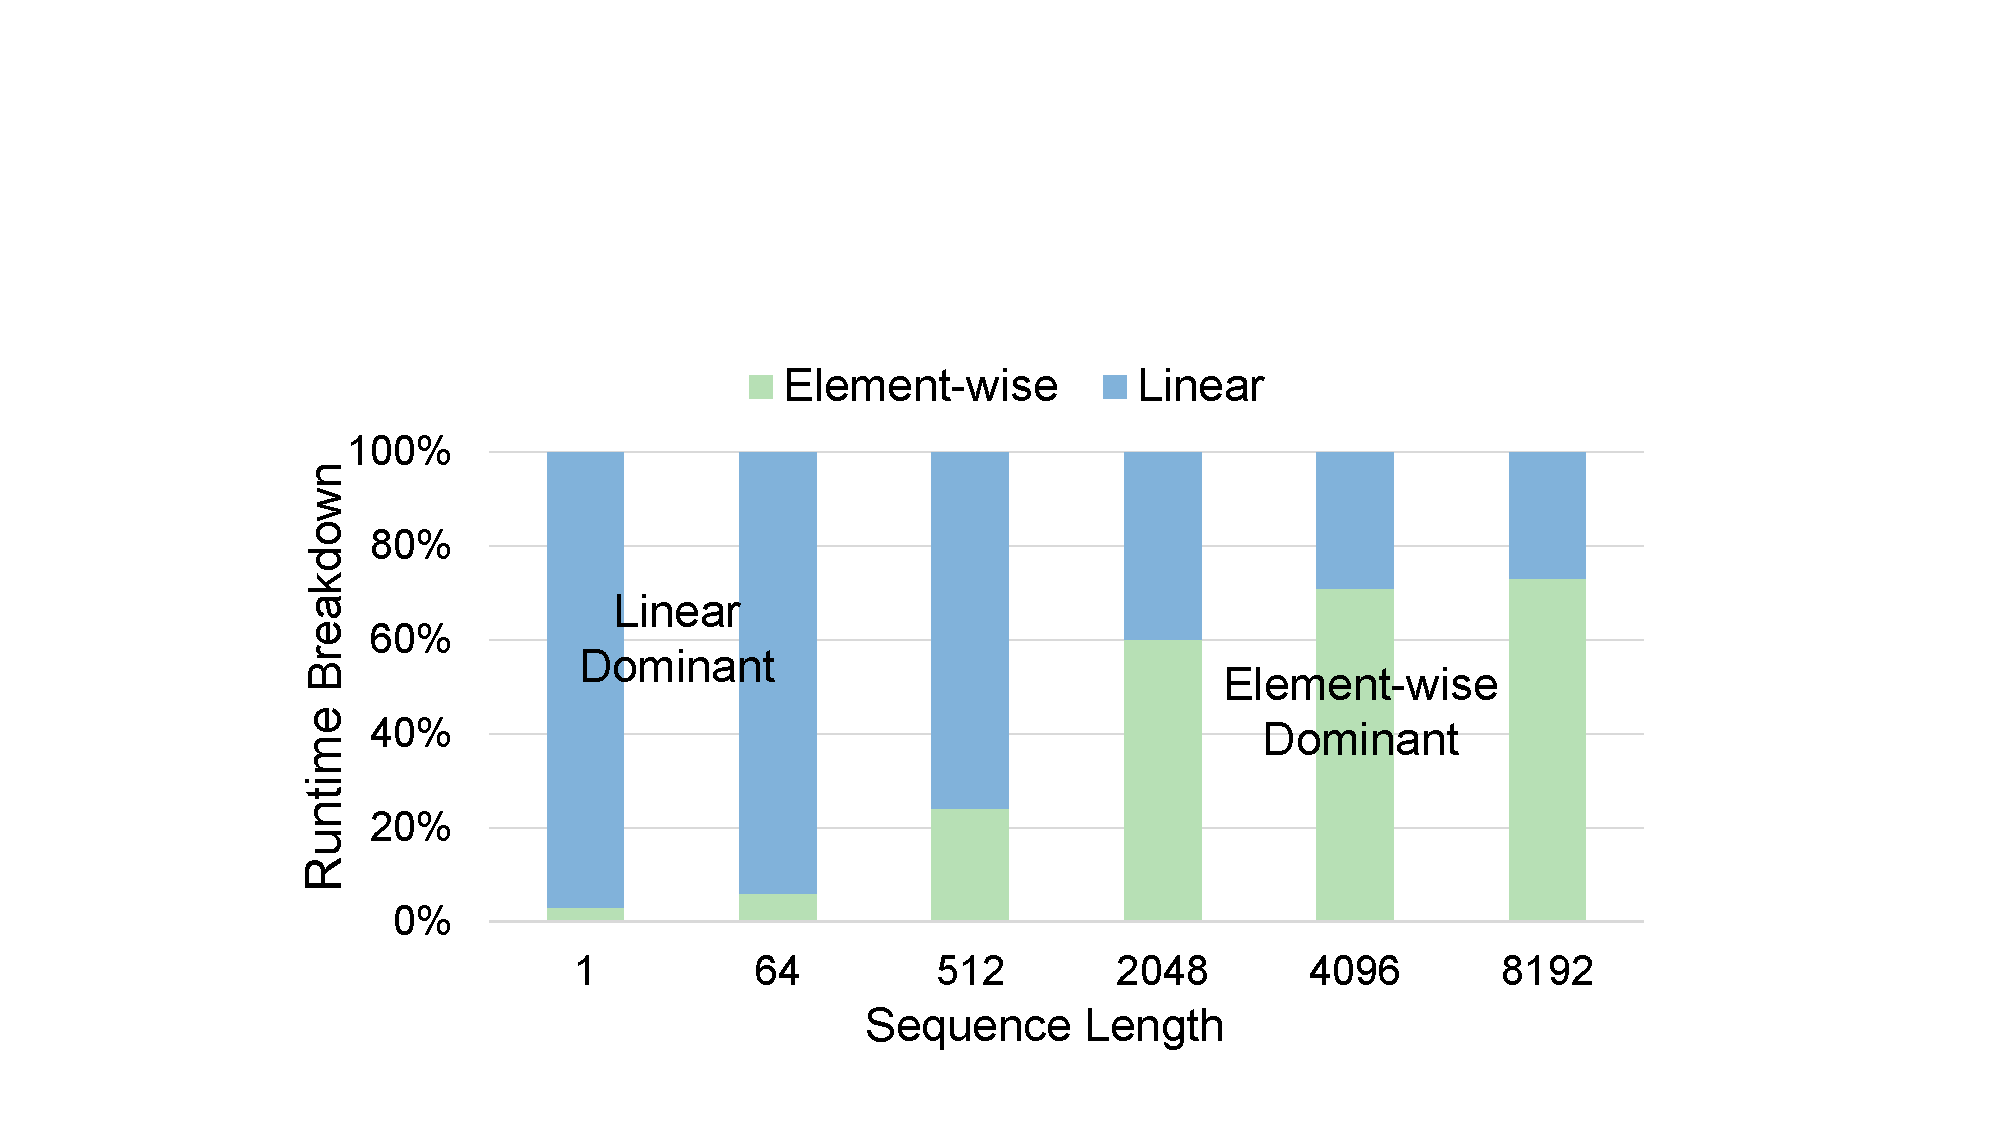
\includegraphics[width=0.4\textwidth]{figures/introduction/breakdown.pdf}
%   \vspace{-12pt}
%   \caption{Runtime breakdown with different sequence lengths in Mamba. Element-wise operations contribute a large fraction of the runtime with long sequence length while linear operations are dominant with short length.}
%   \vspace{-18pt}
%   \label{fig:time_proportion}
% \end{figure}

% %图改成linear用input sharing好，但是element-wise不适用
%  \begin{figure*}[!t]
%   \centering
%   \vspace{-5pt}
%   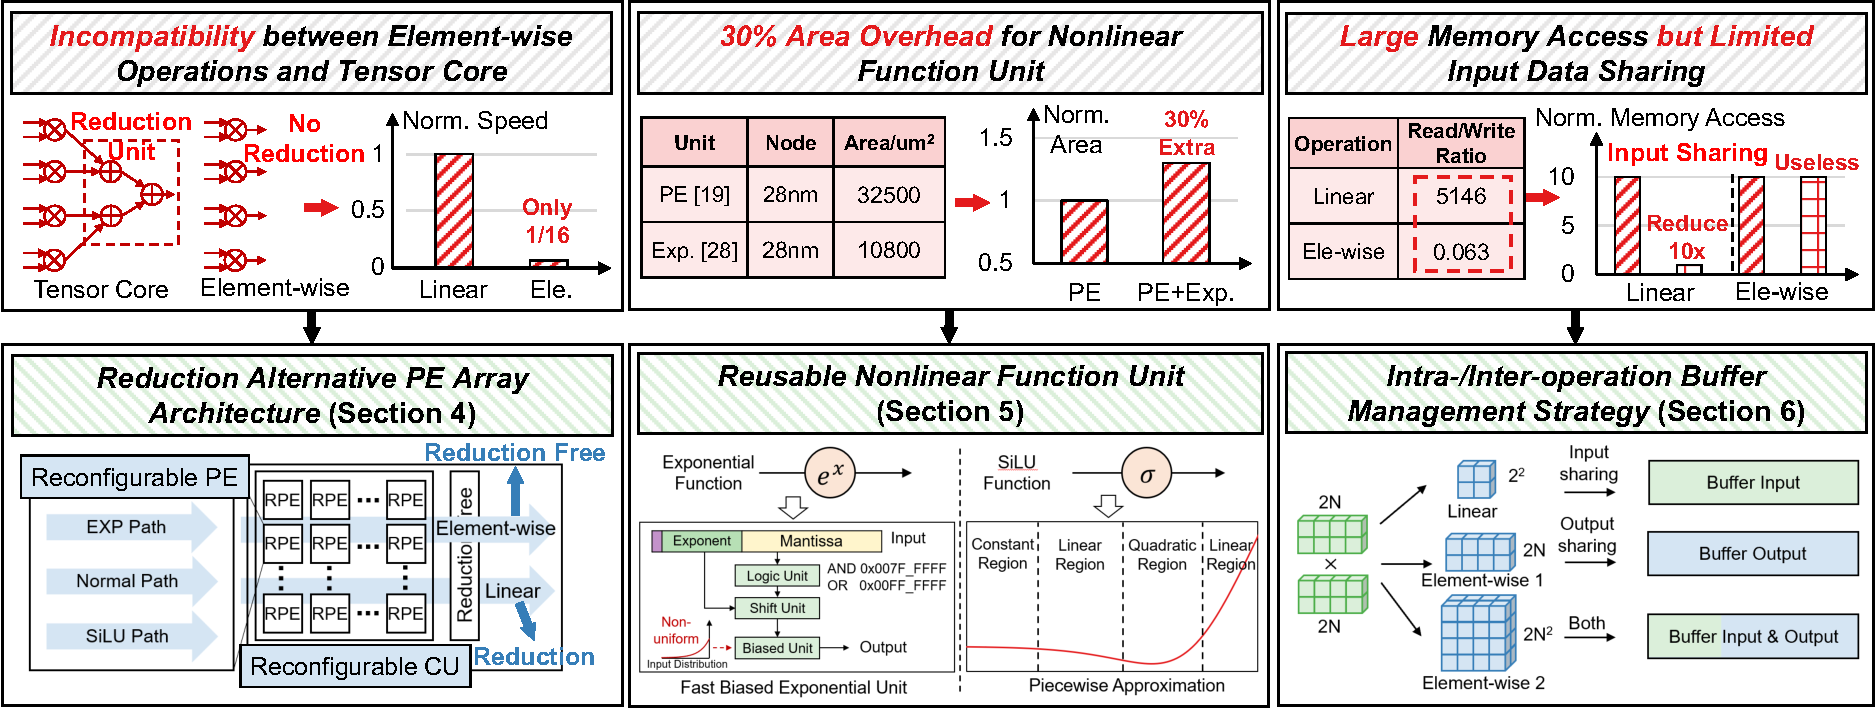
\includegraphics[width=0.98\textwidth]{figures/introduction/overview.pdf}
%   \vspace{-12pt}
%   \caption{Challenges in Mamba computation: (1) incompatibility between element-wise operations and Tensor Core, (2) 30\% area overhead for nonlinear function unit, and (3) large memory access but limited input data sharing for element-wise operations. We propose three novel contributions in \we: (1) reduction alternative PE array architecture, (2) reusable nonlinear function unit, and (3) intra-operation and inter-operation buffer management strategy, to solve these challenges.}
%   \vspace{-15pt}
%   \label{fig:overview}
% \end{figure*}

% However, there is limited research on optimizing for Mamba processing.
% Therefore, we profile the processing carefully and identify three main challenges in Mamba computations:
% \textbf{(1) Incompatibility between element-wise operations and Tensor Core.}
% Linear operations (\textit{e.g.}, matrix multiplication and convolution) and element-wise operations are two dominating operations in Mamba.
% Tensor Core~\cite{tensorcore_a100,tensorcore_h100} is a typical domain specific architecture with reduction tree focused on accelerating these linear operations with high the compute intensity (\textit{e.g.}, $>$1000 FLOPs/Byte).
% However, as shown in Figure~\ref{fig:time_proportion}, the time proportion of element-wise operations escalates significantly as sequence length increases (\textit{e.g.}, $>$60\% with 2048 input length).
% Because the element-wise operations do not need reduction, applying them on Tensor Core-based architecture should introduce large amount of invalid computations, leading to an extreme inefficiency (\textit{e.g.}, 1/16 normalized speed). 
% \textbf{(2) Large area overhead for nonlinear function unit.}
% Exponential function and Sigmoid Linear Unit (SiLU) function are two nonlinear functions in Mamba. Previous methods~\cite{exp_unit,nilsson2014hardware,reggiani2023flex} often design specific unit to compute them, leading to much more area overheads. 
% As shown in Figure~\ref{fig:overview} middle bottom, the optimized nonlinear function unit such exponential function still occupy 30\% of the PE area~\cite{tstc,exp_unit}.
% \textbf{(3) Large memory access but limited input data sharing for element-wise operations.}
% Linear and element-wise operations in Mamba exhibit large compute intensity variance (\textit{e.g.}, $\sim$3 orders of magnitude) and large read/write ratio variance (\textit{e.g.}, $>$3 orders of magnitude). 
% Due to the limited data sharing in element-wise operations, it is useless to apply the existed methods like tiling~\cite{li2019coordinated} to element-wise operations.

% In response to these challenges, we propose \we, a Mamba accelerator with reconfigurable architecture, to support fast and energy-efficient Mamba computations. 
% Our contributions are as follows:
% % \begin{itemize}
%     % \item  
    
% \textbf{(1) Reduction alternative PE array architecture} for both linear and element-wise operations.
% For linear operations, the reduction tree connected to PE arrays is enabled and executes the reduction operation.
% For element-wise operations, the reduction tree is disabled and bypasses the results.
    
% % We propose a reconfigurable architecture controlled by instruction with reconfigurable computing units (RCUs) and processing elements (RPEs). Each RCU is controlled by a reduction tree to support both linear and element-wise operations. Each RPE supports element-wise addition, element-wise multiplication, SiLU, and exponential approximation, to efficiently support both linear and element-wise operations in Mamba.
%     % \item  

% \textbf{(2) Reusable nonlinear function unit} based on reconfigurable PE arrays.
% We decompose the exponential function into element-wise operations and a shift operation by a fast biased exponential algorithm.
%  We also decompose the activation function (SiLU) into a range detection and element-wise operations by a piecewise approximation algorithm.
% Thus, the reconfigurable PEs are fully reused to execute nonlinear functions with negligible accuracy loss.
    
% \textbf{(3) Intra-operation and inter operation buffer management strategy.}
% We propose intra-operation and inter-operation buffer management strategy for linear and element-wise operations. 
% For linear operations, the buffer pool is managed as an input buffer to maximize the input data sharing within each operation. 
% For element-wise operations, the buffer pool is managed as an output buffer to maximize the output data sharing between operations. 
%     % \item  


% % \end{itemize}

% We implement \we in \textit{Verilog} and design a cycle-accurate simulator to evaluate \we. 
% We conduct extensive experiments on Mamba with different model sizes (\textit{i.e.}, Mamba-130M to Mamba-2.8B).
% As a result, \we achieves up to 463.22$\times$/11.66$\times$ speedup and up to 9761.42$\times$/242.52$\times$ energy efficiency compared to Intel Xeon 8358P CPU and NVIDIA Tesla A100 GPU implementations, respectively. 

% %TODO:实验效果
% The rest of this paper is organized as follows. 
% Section~\ref{sec:background} introduces the background of SSM and Mamba model for \we. 
% Three proposed approaches corresponding to the challenges are elaborated in Section~\ref{sec:method1}\textendash\ref{sec:method3}. 
% The overview hardware design of the \we is shown in Section ~\ref{}, and the  . 
% Extensive experimental results are shown in Section~\ref{sec:experiment} and Section~\ref{sec:conclusion} concludes this paper.

%SSM很重要，Mamba的优势，对比transformer，应用场景
%Mamba计算中的问题
%contribution